\documentclass[12pt]{article}
\usepackage{amsmath,amsfonts,amssymb,graphicx,authblk}
\usepackage[font={footnotesize,singlespacing},labelfont=bf]{caption}
\usepackage{titlesec,blkarray, bm} 
\usepackage{float,afterpage}
\usepackage[running,mathlines]{lineno}
\usepackage[vmargin=1in,hmargin=1in]{geometry}
\usepackage[authoryear,sort]{natbib}
\usepackage[dvipsnames]{xcolor}
\usepackage[nodisplayskipstretch]{setspace} 
\usepackage{hyperref}
\usepackage[section]{placeins}
\usepackage{gensymb}
\usepackage{enumitem}
\setlist{topsep=.125em,itemsep=-0.15em,leftmargin=0.75cm}
\setlength{\parindent}{0.35in}

\usepackage[sc]{mathpazo} %Like Palatino with extensive math support
\usepackage[subtle]{savetrees}

\usepackage{lineno}
%\renewcommand{\refname}{Literature Cited}
%\renewcommand{\floatpagefraction}{0.9}
%\renewcommand{\topfraction}{0.99}
%\renewcommand{\textfraction}{0.05}

\clubpenalty = 10000
\widowpenalty = 10000

\sloppy 

\usepackage{ifpdf}
\ifpdf
\DeclareGraphicsExtensions{.pdf,.png,.jpg}
\usepackage{epstopdf}
\else
\DeclareGraphicsExtensions{.eps}
\fi

\graphicspath{{/Users/jm200/Library/CloudStorage/Dropbox/Miller Lab/github/POAR-Forecasting/Manuscript/Figures/}}
\newcommand{\tom}[2]{{\color{red}{#1}}\footnote{\textit{\color{red}{#2}}}}
%\doublespacing


%-------------------------------------------------------------------------
\title{Forecasting range shifts of a dioecious plant species under climate change}
\author[1]{Jacob K. Moutouama \thanks{Corresponding author: jmoutouama@.gmail.com}}
\author[2]{Aldo Compagnoni}
\author[1]{Tom E.X. Miller}
\affil[1]{Program in Ecology and Evolutionary Biology, Department of BioSciences, Rice University, Houston, TX USA}
\affil[2]{Institute of Biology, Martin Luther University Halle-Wittenberg, Halle, Germany; and German Centre for Integrative Biodiversity Research (iDiv), Leipzig, Germany}
\date{} % clear date
%\renewcommand\Authands{ and }

\sloppy


%-------------------------------------------------------------------------
\usepackage{Sweave}
\begin{document}
%\SweaveOpts{concordance=TRUE}
\renewcommand{\baselinestretch}{1.2}
\maketitle

\bigskip 
%45 character limit on running head
\noindent\textbf{Running header:} Forecasting range shifts

\bigskip 
\noindent\textbf{Keywords:} climate change, demography, forecasting, matrix projection model, mechanistic models, sex ratio, range limits

\bigskip 
\noindent\textbf{Acknowledgements:} This research was supported by  XX.

\bigskip
\noindent\textbf{Authorship statement:} XXXXX.  

\bigskip 
\noindent\textbf{Data accessibility statement:} All data \citep{dryaddata} used in this paper are  publicly avaialbale. Should the paper be accepted, all computer scripts supporting the results will be archived in a Zenodo package, with the DOI included at the end of the article. During peer review, our data and code are available at \url{https://github.com/jmoutouama/POAR-Forecasting}. 

\bigskip 
\noindent\textbf{Conflict of interest statement:} None.
\newpage
%\SweaveOpts{concordance=TRUE}
\linenumbers
%-------------------------------------------------------------------------
\spacing{1.25}
\section*{Abstract}
%200 word limit for Ecology letter
Rising temperatures and extreme drought events associated with global climate change have triggered an urgent need for predicting species response to climate change.
Currently, the vast majority of theory and models in population biology, including those used to forecast biodiversity responses to climate change ignore the complication of sex structure. 
To address this issue, we developed two contasting climate-driven population matrix models (one that does not account for sex structure and another one that does account for sex structure) using
demographic data of dioecious species (Texas bluegrass), past and future climate (different carbon gas emission scenarios) to forecast and backcast the effect of climate change on range shifts.
Both models predict a sex specific demographic response to climate change.
Female individuals have a demographic advantage (higher vital rate) over males.
Climate change assuming moderate carbon emission has no negative impact on population viability. 
However, high carbon emission will likely alter population viability in dioecious species and will induce a North-West shift in suitable conditions. 
Overall, our work suggest that tracking only the female could lead to an underestimation of the impact of climate change on dioecious species. 
This study provides a framework for predicting the impact of climate on species using population demography. 

%--------------------------------------------------------------------
\newpage
\section*{Introduction}
Rising temperatures and extreme drought events associated with global climate change are leading to increased concern about how species will become redistributed across the globe under future climate conditions \citep{bertrand2011changes,gamelon2017interactions,smith2024extreme}.
Dioecious species (most animals and many plants) might be particularly vulnerable to the influence of climate change because they often display skewed sex ratios that are generated or reinforced by sexual niche differentiation (distinct responses of females and males to shared climate drivers) \citep{Tognetti2012}. 
Accounting for such a niche differentiation within a population is a long-standing challenge in accurately predicting which sex will successfully track environmental change and how this will impact population viability and range shifts \citep{jones1999sex,gissi2023exploring}. 
The vast majority of theory and models in population biology, including those used to forecast biodiversity responses to climate change, ignore the complication of sex structure \citep{pottier2021sexual,ellis2017does}.
As a result, accurate forecasts of colonization-extinction dynamics for dioecious species under future climate scenarios are limited.

% \tom{Climate change can influence dioecious populations via shifts in sex ratio.}{This paragraph is really good but notice that the topic sentence (and much that follows) is largely redundant with the first paragraph. I would suggest creating clearer distinction between paragraphs.} 
% Females and males may respond differently to climate change, especially in species where there is sexual niche differentiation \citep{gissi2023exploring,gissi2023sex,hultine2016climate}. 
% This sex-specific response to climate change may help one sex to succeed in extreme climatic conditions rather than the other sex \citep{zhao2012sex, burli2022environmental} leading to a skewness in the operational sex ratio (relative number of males and females as available mates) \citep{eberhart2017sex}.
% For example, experiments in two populations of Atlantic marine copepods (\textit{Acartia tonsa}) revealed that male survival was more sensitive to increasing temperatures than female survival \citep{sasaki2019complex}.
% In other species, such as \textit{Pteropus poliocephalus} or \textit {Populus cathayana}, females showed lower survival than males in response to high temperature \citep{welbergen2008climate,zhao2012sex}. 
% Sex-specific responses to climate drivers have the potential to influence population viability under global change because skew in the operational sex ratio can limit reproduction through mate scarcity \citep{petry2016sex}.

Species's range limits, when not driven by dispersal limitation, should generally reflect the limits of the ecological niche \citep{lee2016synthesis}. 
For most species, niches and geographic ranges are often limited by climatic factors including temperature and precipitation \citep{sexton2009evolution}. 
Therefore, any substantial changes in the magnitude of these climatic factors in a given location across the range could impact population viability, with implications for range shifts based on which regions become more or less suitable  \citep{davis2001range, pease1989model}. 
Forecasting range shifts for dioecious species is complicated by the potential for each sex to respond differently to climate variation \citep{pottier2021sexual,morrison2016causes}.
Populations in which males are rare under current climatic conditions could experience low reproductive success due to sperm or pollen limitation that may lead to population decline in response to climate change that disproportionately favors females \citep{eberhart2017sex}.
In contrast, climate change could expand male habitat suitability (e.g. upslope movement), which might increases seed set for pollen-limited females and favor range expansion \citep{petry2016sex}.
Although the response of species to climate warming is an urgent and active area of research, few studies have disentangled the interaction between sex and climate drivers to understand their combined effects on population dynamics and range shifts.  

Our ability to track the impact of climate change on the population dynamics of dioecious plants and the implication of such impact on range shift depends on our ability to build mechanistic models that take into account the spatial and temporal context in which sex specific response to climate change affects population viability \citep{davis2001range,evans2016towards,czachura2020demographic}.
Structured models that are built from long-term demographic data collected from common garden experiments have emerged as powerful technic to study the impact of climate change on species range shift \citep{merow2017climate,schwinning2022common}.
These structured models are increasingly utilized for several reasons. 
First, structured models enable the manipulation of treatments that can isolate spatial and temporal correlations between environmental factors, thus overcoming a main disadvantage with many types of correlative studies \citep{leicht2007comparative}. 
Second, structured models link individual-level demographic trait to population demography allowing the investigation of the demographic mechanisms behind vital rates (e.g. survival, fertility, growth and seed germination) response environmental variation \citep{louthan2022climate,dahlgren2016demography}. 
Third, these structured models can be used to identify which aspect of climate is more important for population dynamics.
For example, Life Table Response Experiment (LTRE) build from structured models is an approach that has become widely used to understand how a given treatment (eg. temperature or precipitation) could affect population dynamics \citep {caswell1989analysis,o2024nonlinear,morrison2007demographic,iler2019reproductive}. 
% At their range edge where climatic conditions are expected to be less favorable, if dioecious species populations are non-viable in response to climate change, global warming will induce range contraction in dioecious species.
% In reverse, if populations at the edge are viable habitats in response to global warming, dioecious species populations could shift their range and relocate to more favorable and thereby favored range expansion. 

In this study, we used a mechanistic approach by combining geographically-distributed field experiments, bayesian statistical modeling, and two-sex population projection modeling to understand the demographic response of dioecious species to climate change and its implications for future range dynamics.
Our study system is a dioecious plant species (\textit{Poa arachnifera}) distributed along environmental gradients in the south-central US corresponding to variation in temperature across latitude and precipitation across longitude. 
A previous study on the same system showed that, despite a differentiation of climatic niche between sexes, the female niche mattered the most in driving the environmental limits of population viability \citep{miller2022two}.
However that study did not use climate variables preventing us from backcasting and forecasting the impact of climate change on dioecious species.
Here, we asked four questions: 
\begin{enumerate}
	\item What are the sex-specific vital rate responses to variation in temperature and precipitation across the species' range ?
	\item How sex-specific vital rates combine to determine the influence of climate variation on population growth rate ($\lambda$) ?
	\item What are the historical and projected changes in climate across the species range ?
	\item What are the back-casted and fore-casted dynamics of this species' geographic niche ($\lambda \geq 1$) and how does accounting for sex structure modify these predictions ?
\end{enumerate}

%--------------------------------------------------------------------
\section*{Materials and methods}
\subsection*{Study species}
Texas bluegrass (\textit{Poa arachnifera}) is a dioecious perennial, summer-dormant cool-season (C3) grass that occurs in the south-central U.S. (Texas, Oklahoma, and southern Kansas) \citep{hitchcock1971manual}. 
Average temperatures along the distribution of the species tend to decrease northward as a result of the influence of latitude: lower latitudes receive more heat from the sun over the course of a year.
Similarly the average precipitation decrease eastward as a result of the influence of longitude: lower longitudes receive less precipitation over the year.
Texas bluegrass grows between October and May (growing season), with onset of dormancy often from June to September (dormant season) \citep{kindiger2004interspecific}.
Flowering occurs in May and the species is wind pollinated \citep{hitchcock1971manual}.
% {\color{blue} The male heads are smooth, while those of the female appear fuzzy.}

\subsection*{Common garden experiment}
We set up a common garden experiment throughout and beyond the range of Texas bluegrass to enable study of sex-specific demographic responses to climate and the implications for range shifts. 
The novelty of this study lies in the fact that we use a precise climate variable to build a mechanistic model to forecast the response of species to climate change.
Details of the experimental design are provided in \cite{miller2022two}; we provide a brief overview here. 
The common experiment was installed at 14 sites across a climatic gradient (Fig.\ref{fig:study_design}.
At each site, we established 14 blocks. 
For each block we planted three female and three male individuals that were clonally propagated from eight natural source populations of Texas bluegrass. 
The experiment was established in November 2013 and was census annually through 2016, providing both spatial and inter-annual variation in climate. 
Each May (2014-2016), we collected individual demographic data including survival (alive or dead), growth (number of tillers), flowering status (reproductive or vegetative), and fertility (number of panicles, conditional on flowering). 
For the analyses that follow, we focus on the 2014-15 and 2015-16 transitions years.

\begin{figure}[H]
  \begin{center}
    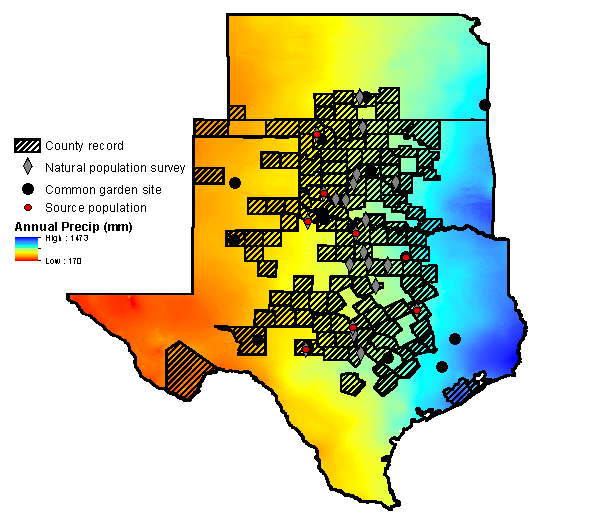
\includegraphics[width=0.90\linewidth]{Figures/POAR_BONAP_survey_garden_map.pdf}
  \caption{XXX}
  \label{fig:study_design}
  \end{center}
\end{figure}

\subsection*{Climatic data collection}
We downloaded monthly temperature and precipitation from Chelsa to describe observed climate conditions during our study period \citep{karger2017climatologies}.
These climate data were used as covariates in vital rate regressions, which allowed us to forecast and back-cast demographic responses to climate change based on observations across the common garden experiment. 
%We prefer temperature and precipitation because they capture the most the climate in the study region \colorbox{BurntOrange}{Source}. 
We aligned the climatic years to match demographic transition years \tom{(May 1 -- April 30)}{I am not sure if these are actually the right dates.} rather than calendar years.
Based on the natural history of this summer-dormant cool-season species, we divided each transition year into growing and dormant seasons. 
We define June through September as the dormant season and the rest of the year as the growing season. 
Across years and sites, the experiment included substantial variation in growing and dormant season temperature and precipitation (Supporting Information \ref{Sup:pr_variation}, \ref{Sup:temp_variation}).

To back-cast and forecast changes in climate, we downloaded projection data for three 30-year periods: past (1901-1930), current (1990-2019) and future (2070-2100).
Data for these climatic periods were downloaded from four general circulation models (GCMs) selected from the Coupled Model Intercomparison Project Phase 5 (CMIP5). 
The GCMs are MIROC5, ACCESS1-3, CESM1-BGC, CMCC-CM  and were downloaded from chelsa \citep{sanderson2015representative}.
We evaluated future climate projections from two scenarios of representative concentration pathways (RCPs): RCP4.5, an intermediate-to-pessimistic scenario assuming a radiative forcing to amount to 4.5 $W m^{-2}$ by 2100, and RCP8.5, a pessimistic emission scenario which project a radiative forcing to amount to 8.5 $W m^{-2}$ by 2100 \citep{thomson2011rcp4, schwalm2020rcp8}.

\subsection*{Sex ratio experiment}
We conducted a sex-ratio experiment on a site close (1 km) to a natural population of the focal species at the center of the range to estimate the effect of sex-ratio variation on female reproductive success.
Details of the experiment are provided in \cite{compagnoni2017can} and \cite{miller2022two}.
In short, we established 124 experimental populations on plots measuring 0.4 x 0.4m and separated by at least 15m from each other at that site. 
We chose 15m because our pilot data show that more than 90\% of wind pollination occurred within 13m. 
We varied population density (1-48 plants/plot) and sex ratio (0\%-100\% female) across the experimental populations, and we replicated 34 combinations of density-sex ratios. 
We collected the number of panicles from a subset of females in each plot and collected the number of seeds in each panicle.
Since the number of panicles (proxy of reproduction effort) does not necessarily reflect reproduction success in \textit{Poar arachnifera}, we accessed reproduction success (seed fertilized) using greenhouse-based germination and trazolium-based seed viability assays. 

We used the sex-ratio to estimate the probability of viability and the germination rate. 
Seed viability was modeled with a binomial distribution where the probability of viability ($v$) was given by:
\begin{align}\label{eq:viab_fn}
v = v_{0} * (1 - OSR^{\alpha})
\end{align}
\noindent where $OSR$ is the operational sex ratio (proportion of panicles that were female) in the experimental populations.
The properties of the above function is supported by our previous work \citep{compagnoni2017can}. 
Here, seed viability is maximized at $v_{0}$ as $OSR$ approaches zero (strongly male-biased) and goes to zero as $OSR$ approaches $1$ (strongly female-biased).
Parameter $\alpha$ controls how viability declines with increasing female bias.

We used a binomial distribution to model the germination data from greenhouse trials.
Given that germination was conditional on seed viability,the probability of success was given by the product $v*g$, where $v$ is a function of $OSR$ (Eq. \ref{eq:viab_fn}) and $g$ is assumed to be constant.

\subsection*{Sex specific demographic responses to climate}
We used individual level measurements of survival, growth (number of tillers), flowering, number of panicles to independently develop Bayesian mixed effect models describing how each vital rate varies as a function of sex, size, precipitation of growing and dormant season and temperature of of growing and dormant season. 
We fit vital rate models with second-degree polynomial functions for the influence of climate.
We included a second-degree polynomial because we expected that climate variables would affect vital rates through a hump-shaped relationship. 

We centered and standardized all climatic predictors to facilitate model convergence.
However, Size was on a natural logarithm scale. 
We included site,source, and block as random effect.
All the vital rate models used the same linear and quadratic predictor for the expected value ($\mu$)(Eq.\ref{eq:mu}) . 
However, we applied a different link function ($f(\mu)$) depending on the distribution the vital rate. 
We modeled survival and flowering data with a Bernoulli distribution.
We modeled the growth (tiller number) with a zero-truncated Poisson inverse Gaussian distribution. 
Fertility (panicle count) was model as zero-truncated negative binomial. 
\begin{align}\label{eq:mu}
\begin{split}
f(\mu) = \beta_{0} + \beta_{1}size + \beta_{2}sex + \beta_{3}pptgrow + \beta_{4}pptdorm + \beta_{5}tempgrow + \beta_{6}tempdorm \\ 
+ \beta_{7}pptgrow*sex + \beta_{8}pptdorm*sex + \beta_{9}tempgrow*sex + \beta_{10}tempdorm*sex  \\ 
+  \beta_{11}size*sex + \beta_{12}pptgrow*tempgrow + \beta_{13}pptdorm*tempdorm\\
+ \beta_{14}pptgrow*tempgrow*sex + \beta_{15}pptdorm*tempdorm*sex + \beta_{16}pptgrow^2\\
+ \beta_{17}pptdorm^2 + \beta_{18}tempgrow^2 + \beta_{19}tempdorm^2 + \beta_{20}pptgrow^2*sex  \\
+ \beta_{21}pptdorm^2*sex + \beta_{22}tempgrow^2*sex + \beta_{23}tempdorm^2*sex + \phi + \rho + \nu 
\end{split}
\end{align}
\noindent where $\beta_{0}$ is the  grand mean intercept, $\beta_{1}$ is the size dependent slopes.
$size$ was on a natural logarithm scale. 
$\beta_{2}$...$\beta_{13}$ represent the climate dependent slopes.
$\beta_{14}$...$\beta_{23}$ represent the sex-climate interaction slopes.
$pptgrow$ is the precipitation of the growing season (standardized to mean zero and unit variance), $tempgrow$ is the temperature of the growing season (standardized to mean zero and unit variance), $pptdorm$ is the precipitation of the dormant season (standardized to mean zero and unit variance), $tempdorm$ is the temperature of the dormant season (standardized to mean zero and unit variance).
The model also includes normally distributed random effects for block-to-block variation ($\phi \sim N(0,\ \sigma_{block})$) and source-to-source variation that is related to the provenence of the seeds used to establish the common garden ($\rho \sim N(0,\ \sigma_{source})$), site to site variation ($\nu \sim N(0,\ \sigma_{site})$).
We fit survival, growth, flowering models with generic weakly informative priors for coefficients ($\mu = 0,\ \sigma = 1.5$) and variances ($\gamma [0.1,\ 0.1]$).
{\color{blue}We fit fertility model with regularizing priors for coefficients ($\mu = 0,\ \sigma = 0.15$).} 
% because the models could not converge with the same priors that was used for he other vital rates.
We ran three chains for 1000 samples for warmup and 4000 for interactions, with a thinning rate of 3.
We accessed the quality of the models using trace plots and predictive check graphs \citep{piironen2017comparison} (Supporting Information \ref{Sup:PPC}).
To understand the effect of climate on vital rates, we got the 95 \% credible interval of the posterior distribution.  
Then we assumed that there is 95 \% probability that the true (unknown) estimates would lie within that interval, given the evidence provided by the observed data for each vital rate.
All models were fit in Stan \citep{rstan}. 

\subsection*{Influence of climate variation on population growth rate}
To understand the effect of climate on population growth rate, we used the vital rate estimated earlier to build a matrix projection model (MPM) structured by size (number of tillers), sex and climate (dormant and growing) as covariate.  
Let $F_{x,z,t}$ and $M_{x,z,t}$ be the number of female and male plants of size $x$ in year $t$ present at a location that has $z$ as climate, where $x \in \{1,2,...,U\}$ and $U$ is the maximum number of tillers a plant can reach (here 95th percentile of observed maximum size).
Let $F^{R}_{t}$ and $M^{R}_{t}$ be the new recruits, which we assume do not reproduce in their first year.
We assume that the parameters of sex ratio-dependent mating (Eq. \ref{eq:viab_fn}) do not vary with climate.  
For a pre-breeding census, the expected numbers of recruits in year $t+1$ is given by:
\begin{align}\label{eq:recruits}
F^{R}_{t+1} = \sum_{x=1}^{U} 	[ \, p^{F}(x,z) \cdot c^{F}(x,z) \cdot d \cdot v(\mathbf{F_{t}},\mathbf{M_{t}}) \cdot m \cdot \rho 	] \, F_{x,z,t}
\\
M^{R}_{t+1} = \sum_{x=1}^{U} 	[ \, p^{F}(x,z) \cdot c^{F}(x,z) \cdot d \cdot v(\mathbf{F_{t}},\mathbf{M_{t}}) \cdot m \cdot (1-\rho) 	] \, F_{x,z,t}
\end{align}

\noindent where $p^{F}$ and $c^{F}$ are flowering probability and panicle production for females of size $x$, $d$ is the number of seeds per female panicle, $v$ is the probability that a seed is fertilized, $m$ is the probability that a fertilized seed germinates, and $\rho$ is the primary sex ratio (proportion of recruits that are female), $z$ is the climate. 
Seed fertilization depends on the OSR of panicles (following Eq. \ref{eq:viab_fn}) which was derived from the $U \times 1$ vectors of population structure $\mathbf{F_{t}}$ and $\mathbf{M_{t}}$:
\begin{align}\label{eq:viab_MPM}
v(\mathbf{F_{t}},\mathbf{M_{t}}) = v_{0} * \left[ 1 - \left( \frac{\sum_{x=1}^{U} p^{F}(x,z) c^{F}(x,z) F_{x,z,t}}{\sum_{x=1}^{U} p^{F}(x,z) c^{F}(x,z) F_{x,z,t} + p^{M}(x,z) c^{M}(x,z) M_{x,z,t}} \right) ^{\alpha}\right]
\end{align}

Thus, the dynamics of the size-structured component of the population are given by:
\begin{align}\label{eq:dynamics}
F_{y,t+1} = [ \, \sigma \cdot g^{F}(y,x=1,z) ] \, F^{R}_{t} + \sum_{x=1}^{U} 	[ \, s^{F}(x,z) \cdot g^{F}(y,x,z)] \, F_{x,z,t}
\\
M_{y,t+1} = [ \, \sigma \cdot g^{M}(y,x=1,z) ] \, M^{R}_{t} + \sum_{x=1}^{U} 	[ \,  s^{M}(x,z) \cdot g^{M}(y,x,z) ] \, M_{x,z,t}
\end{align}

\noindent In the two formula above, the first term indicates seedlings that survived their first year and enter the size distribution of established plants.
Instead of using \textit{P. arachnifera} survival probability, we used the seedling survival probability ($\sigma$) from demographic studies of the hermaphroditic congener \textit{Poa autumnalis} in east Texas (T.E.X. Miller and J.A. Rudgers, \textit{unpublished data}), and we assume this probability was constant across sexes and climatic variables. 
We did this because we had little information on the early life cycle transitions of greenhouse-raised transplants.
We also assume that $g(y,x=1)$ is the probability that a surviving seedlings reach size $y$, the expected future size of 1-tiller plants from the transplant experiment.
The second term represents survival and size transition of established plants from the previous year, where $s$ and $g$ give the probabilities of surviving at size $x$ and growing from sizes $x$ to $y$, respectively, and superscripts indicate that these functions may be unique to females ($F$) and males ($M$).

Since the two-sex MPM is nonlinear (vital rates affect and are affected by population structure) we estimated the asymptotic geometric growth rate ($\lambda$) by numerical simulation, and repeated this across a range of climate.

\subsection*{Identifying the mechanisms of population growth rate sensitivity to climate }
To identify which aspect of climate is most important for population viability, we used a "random design" Life Table Response Experiment (LTRE). 
We used the RandomForest package to fit a regression model with $\theta$ as predictors  and $\lambda$ as response \citep{ellner2016data,liaw2002classification}.
The LTRE approximates the variation in $\lambda$ in response to climate covariates and their interaction \citep{caswell2000matrix,hernandez2023exact}:
\begin{align}\label{eq:ltre}
Var(\lambda_{c})\approx \sum_{i=-1}^{n}\sum_{j=1}^{n} Cov(\theta_{i},\theta_{j},\theta_{ij}) + Var (\epsilon)
\end{align}

\noindent where, $\theta_{i}$, $\theta_{j}$, $\theta_{ij}$  represent respectively the fitted regression slope for the covariate of the dormant season,j the covariate of the growing season and ij the covariate of their interactions. 

To identify the mechanism by which climate affects population growth rate for each sex, we decomposed the effect of each climate variable (here Climate) on population growth rate ($\lambda$) into contribution arising from the effect on each stage-specific vital rate \citep{caswell2000matrix}.
At this end we used a life table response experiment (LTRE) with a regression designs. 
The LTRE approximates the change in $\lambda$ with climate  as the product of the sensitivity of $\lambda$ to the parameters times the sensitivity of the parameters to climate, summed over all parameters \citep{caswell1989analysis}:
\begin{align}\label{eq:ltresex}
\frac{\partial \lambda}{\partial Climate} \approx \sum_{i} \frac{\partial \lambda}{\partial \theta^{F}_{i}} \frac{\partial \theta^{F}_{i}}{\partial Climate} + \frac{\partial \lambda}{\partial \theta^{M}_{i}} \frac{\partial \theta^{M}_{i}}{\partial Climate}
\end{align}

\noindent where, $\theta^{F}_{i}$ and $\theta^{M}_{i}$ represent sex-specific parameters: the regression coefficients for the intercepts and slopes of size-dependent vital rate functions. 
Because LTRE contributions are additive, we summed across vital rates to compare the total contributions of female and male parameters. 

\subsection*{Impact of climate change on niche and range shifts}
A species' ecological niche can be defined as the range of resources and conditions (physical and environmental) allowing the species to maintain a viable population ($\lambda \geq 1$).
To understand the impact of climate change on species niche shifts, we estimated the probability of  population viability being greater than  1, Pr ($\lambda > 1$) conditional to two environmental axes \citep{diez2014probabilistic}.
Because the study species is a cool season grass species, we used two environmental axes: (1) temperature and precipitation of the dormant season and (2) temperature and precipitation of the growing season. 
Pr ($\lambda > 1$) was calculated using the proportion of the Markov chain Monte Carlo iterations (here, 300) that lead to a $\lambda > 1$
Population viability-environment relationship was mapped onto geographic layers of three state (Texas, Oklahoma and Kansas) to delineate past, current and future potential distribution of the species.
To do so, we estimated Pr ($\lambda > 1$) as a function of all climate covariates for each pixel (1km*1km) across the species range using the posterior distribution. 
Because of amount of the computation involve in the Markov chain Monte Carlo iterations, use only 100 posterior samples to estimate Pr ($\lambda > 1$) across the Texas, Oklahoma and Kansas.

% All the analysis were performed in R 4.3.1 \citep{RCoreteam}
All calculations were processed in parallel using open-source software on the Rice Super computer (NOTS) and the German Centre for Integrative Biodiversity Research (iDiv) High-Performance Computing (HPC) Cluster. {\color{blue} This was achieved by splitting the global point occurrence records sent to single computational node}. 



\section*{Results}
\subsection*{Sex specific demographic response to climate change}
Most vital rates were strongly climate dependent, but the magnitude of their response differed between sexes suggesting a sex-specific demographic response to climate. 
Survival and flowering were strongly more dependent on climate than growth (number of tillers) and reproduction (number of panicles) (Fig.\ref{fig:vital_rates}; Supporting Information \ref{Sup:Posterior}).
In addition, we found opposite patterns in the direction of the effect on seasonal climate on the probability of survival and flowering.
The growing season (precipitation) has a negative effect on the probability of survival, number of tillers, and the probability of flowering, whereas the dormant season has a positive effect on these vital rates. 
Unlike precipitation, temperature had different effects on different vital rates.
Temperature of the growing season has a positive effect of the probability of survival, a negative effect of the probability of flowering, and the number of tillers, but no significant effect on the number of panicles. 
Further, there was a female survival and flowering advantage across both climatic seasons (Figures. 3A-3D, 3I-3L). 
On the contrary, there was a male panicle advantage across all climatic variables (Figure3M-3P). 
Counter-intuitively, there was no significant sex growth advantage in all season climatic variables (Figures. 3E-3H). 
Plant size x sex interaction was significant for all vitals rates (Supporting Information \ref{Sup:Posterior}).
For survival, flowering and reproduction the interaction between temperature and precipitation of the growing season and dormant season was not significant (Supporting Information \ref{Sup:Posterior}). 
However, for growth the interaction between temperature and precipitation of the growing season and dormant season was significantly higher than zero (Supporting Information \ref{Sup:Posterior}). 

\begin{figure}[H]
  \begin{center}
    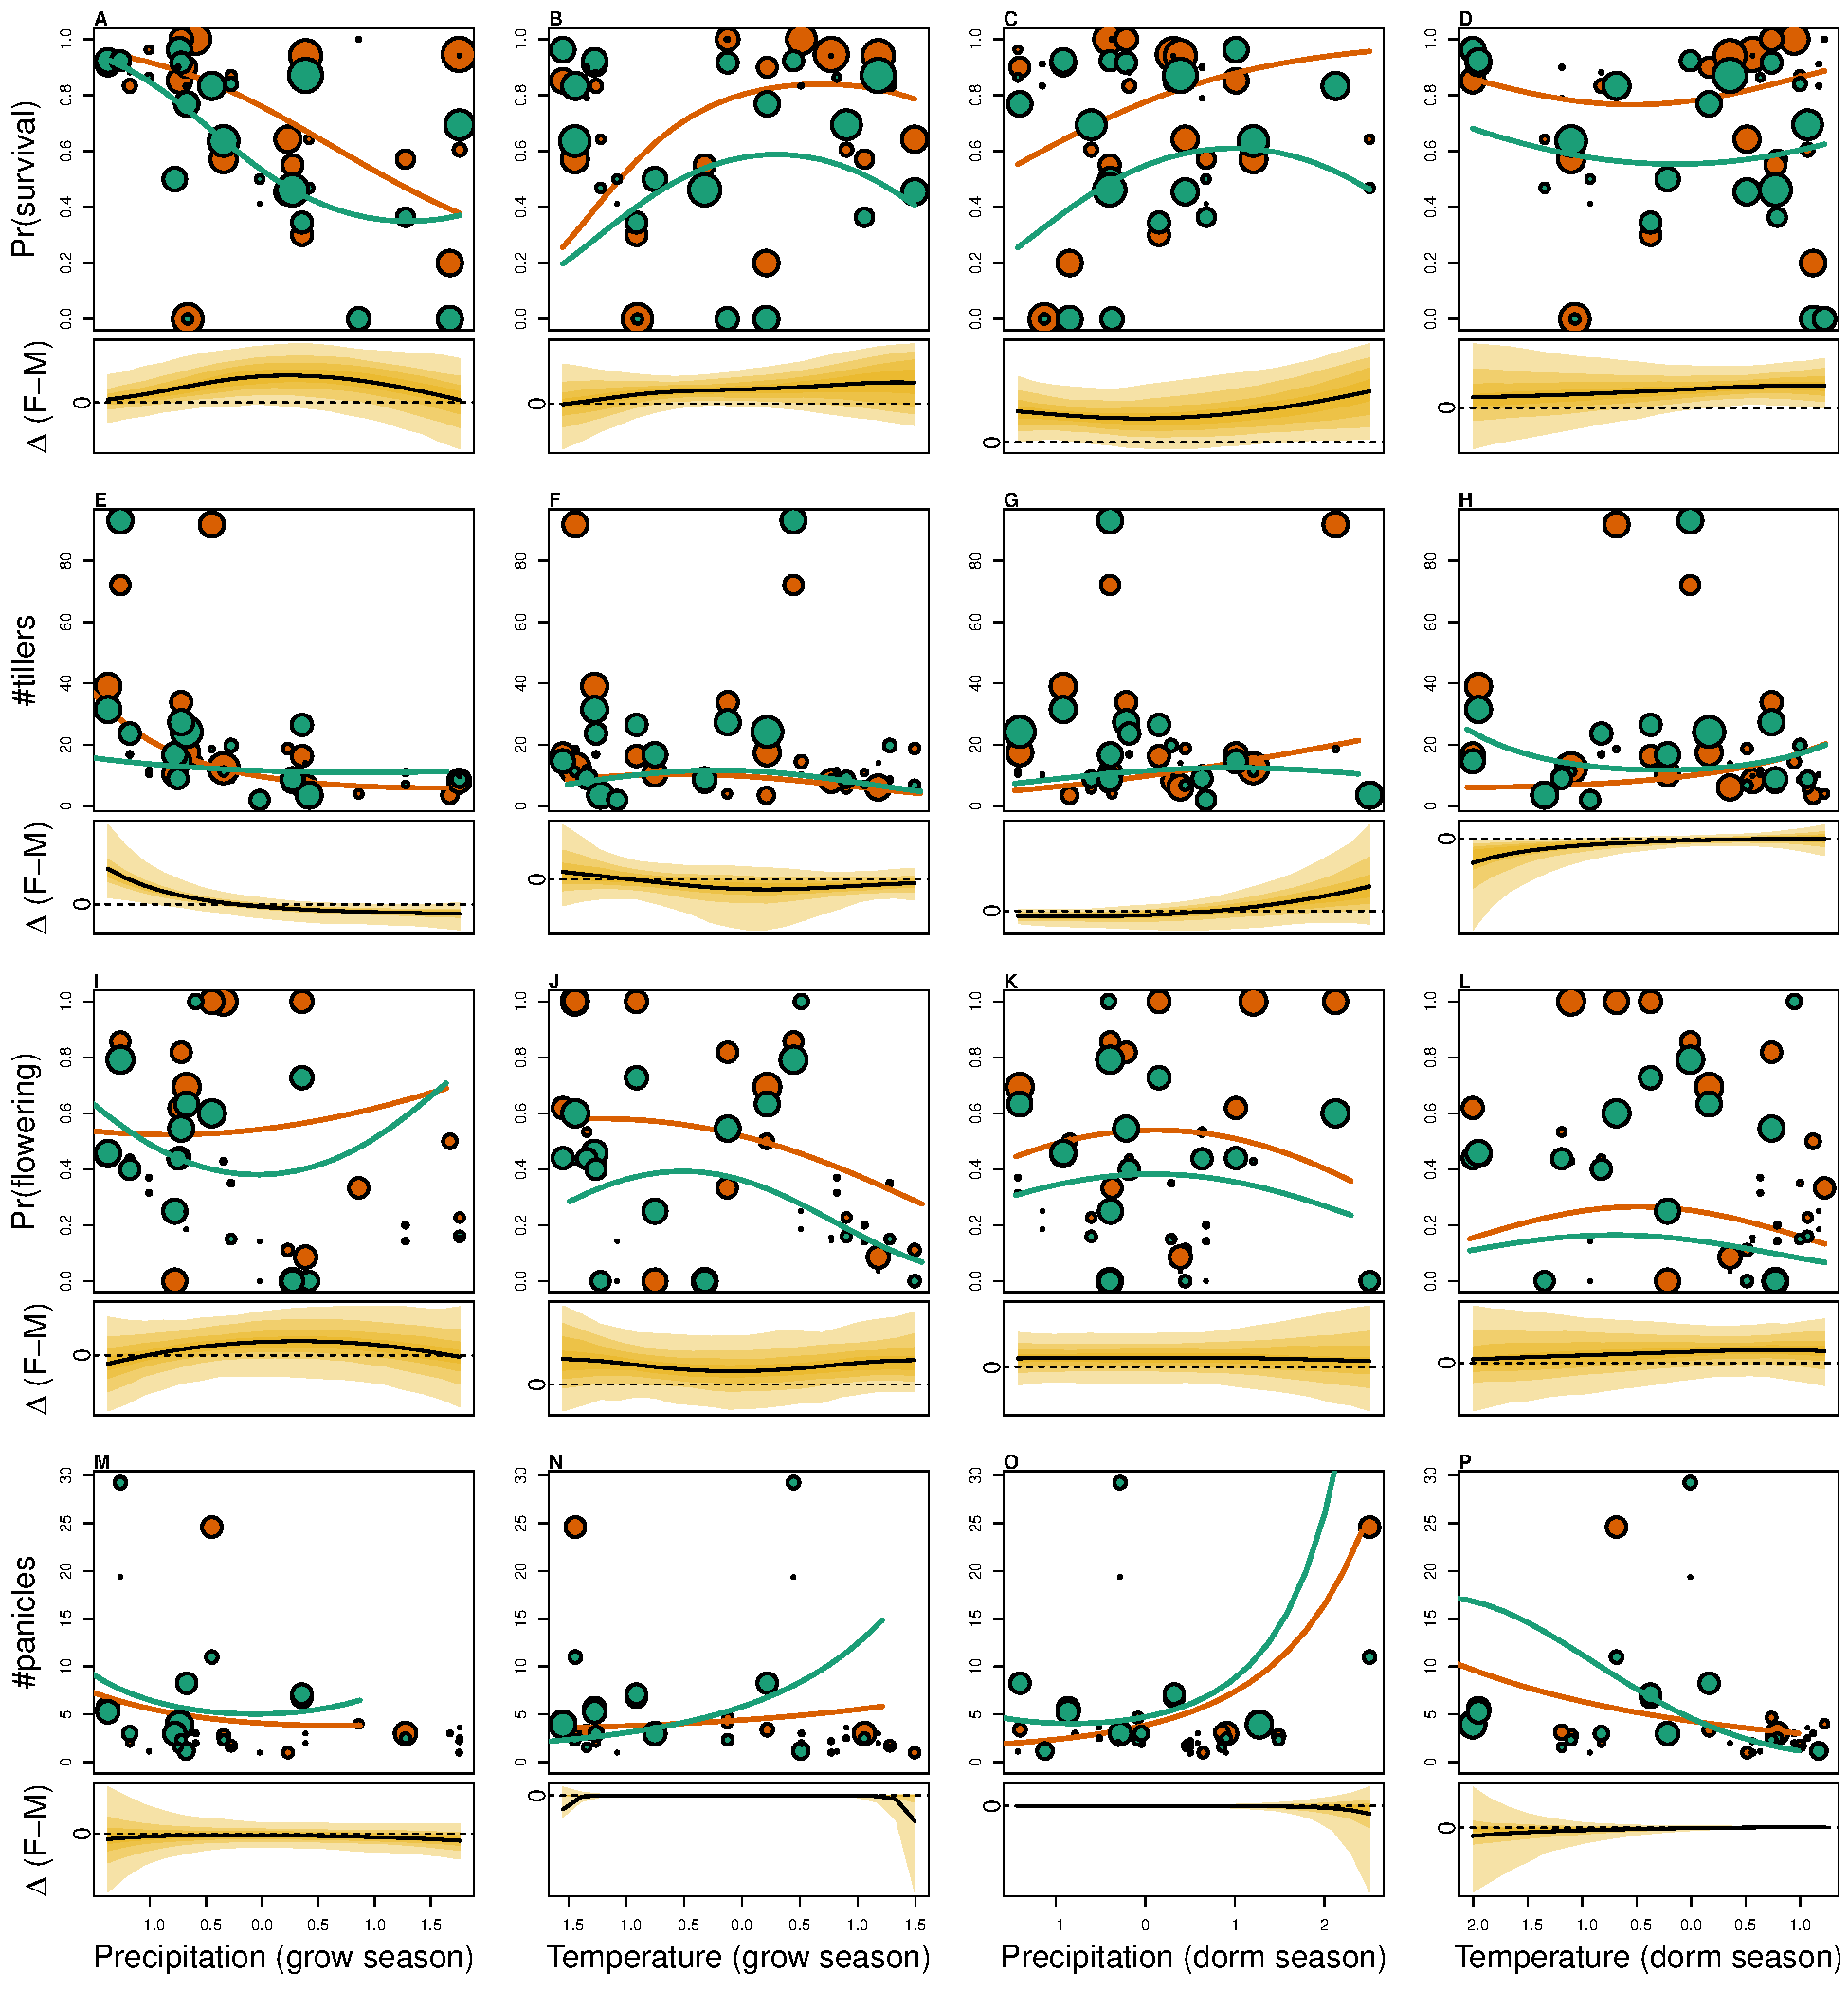
\includegraphics[width=0.95\linewidth]{Figures/vital_rates.pdf}
  \caption{Sex specific demographic response to climate across species range: A--D, inter-annual probability of survival; E--H, inter-annual growth (change in number of tillers); I--L, probability of flowering; M--P, number of panicles produced given flowering. 
  Points show means by site for females (orange) and males (green). 
  Point size is proportional to the sample size of the mean.
  Lines show fitted statistical models for females (orange) and males (green) based on posterior mean parameter values.
  Lower panels below each data panel show the posterior distribution of the difference between females and males as a function of climate (positive and negative values indicate female and male advantage, respectively); dashed horizontal line shows zero difference.}
  \label{fig:vital_rates}
  \end{center}
\end{figure}

\subsection*{Climate change alter population viability}
We estimated the predicted response of  population growth rate (population fitness) to seasonal climate gradients using a model assuming a female dominant model and another model using the two sexes. 
Consistent with the effect of climate on the individual vital rate, we found a strong effect of seasonal climate on population fitness (Fig.\ref{fig:lambda}). 
For both models (female dominant and two sexes), population fitness decreased with an increase of precipitation of growing season. 
In contrast population fitness increased with precipitation of the dormant season.
Furthermore, population fitness was maximized between 23 and 17 \degree C and decreases to zero just beyond 32 \degree C during the growing season.
Similarly population fitness was maximized between 13 and 17 \degree C and decreases to zero just beyond 20 \degree C during the growing season.
We have also detected a strong effect of the past and future climate on population growth rate. However, for future climate, the magnitude of that effect was different between gas-scenario emissions. 
A moderate emission gas scenario (RCP4.5) has a no effect on the population growth rate while a high emission scenario (RCP8.5) has a strong negative effect on the population growth rate. 
High-emission scenario (RCP8.5) will lead to an alteration of population viability. 
Under past climate conditions, population growth rate decreased below one for temperature of the growing season and the dormant season.

Population viability was most sensitive to change in temperature of the growing season and temperature of the dormant season. 
LTRE decomposition reveals that, for each sex, the reduction of lambda for high value of temperature of the growing season (Northern range) was driven by a reduction of survival rate, growth rate, flowering and a reduction in number of panicles. 
However, the reduction of for higher value of temperature of the dormant season was driven by only the female. 

\begin{figure}[H]
  \begin{center}
    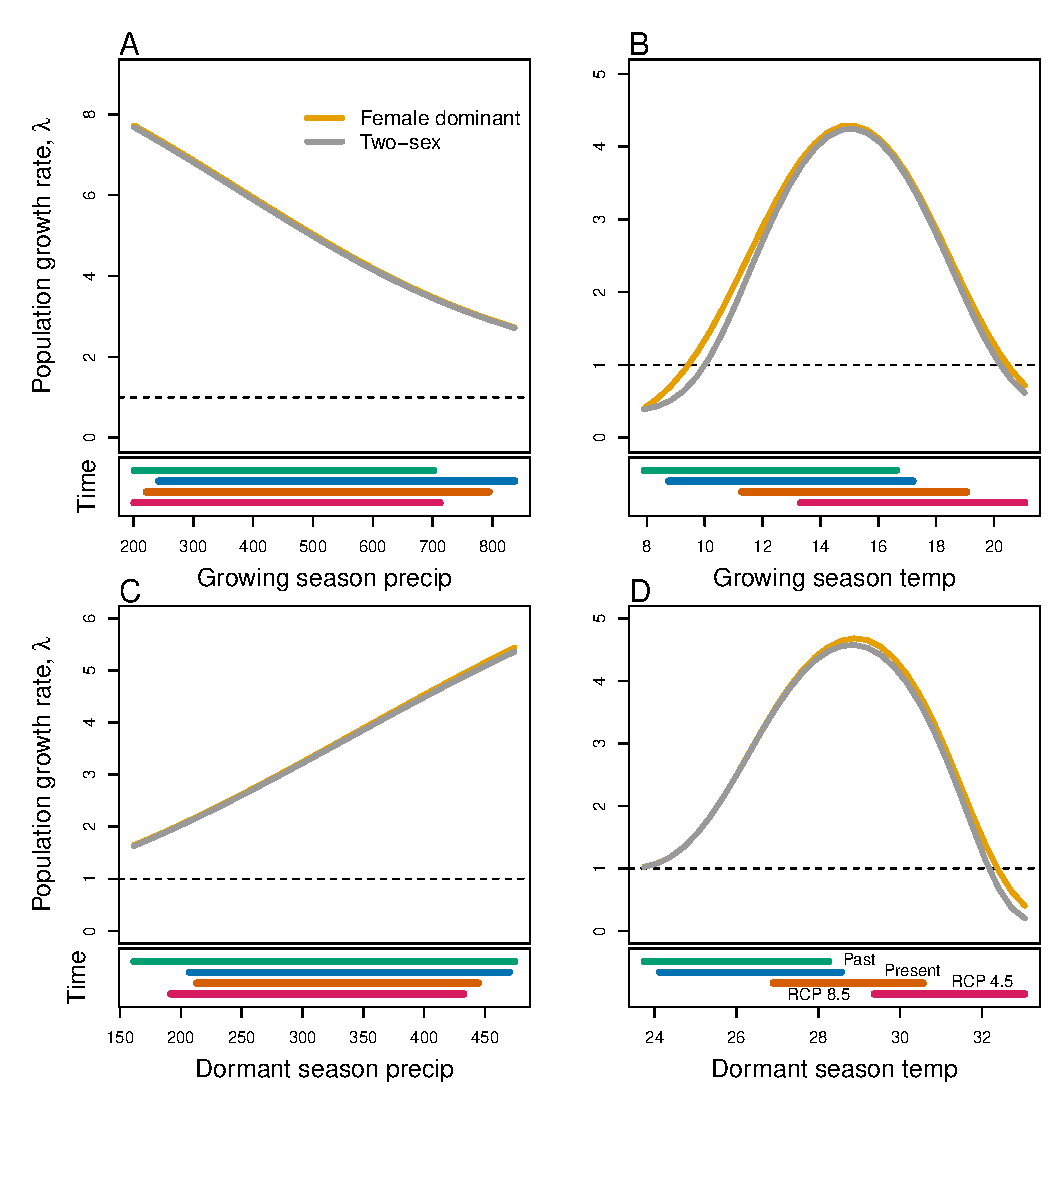
\includegraphics[width=0.95\linewidth]{Figures/lambda_past_present_future.pdf}
  \caption{Population growth rate ($\lambda$) as a function of climate (past climate, present and predicted future climates). For future climate, we show a Representation Concentration Pathways 4.5 and 8.5. Values of ($\lambda$) are derived from the mean climate variables across 4 GCMs. The solid bold curve shows prediction by the two-sex matrix projection model that incorporates sex- specific demographic responses to climate with sex ratio dependent seed fertilization. The bold dashed curve represents the prediction by the female dominant matrix projection model. The dashed horizontal line indicates the limit of population viability ($\lambda$ = 1)}
  \label{fig:lambda}
  \end{center}
\end{figure}


\begin{figure}[H]
  \begin{center}
    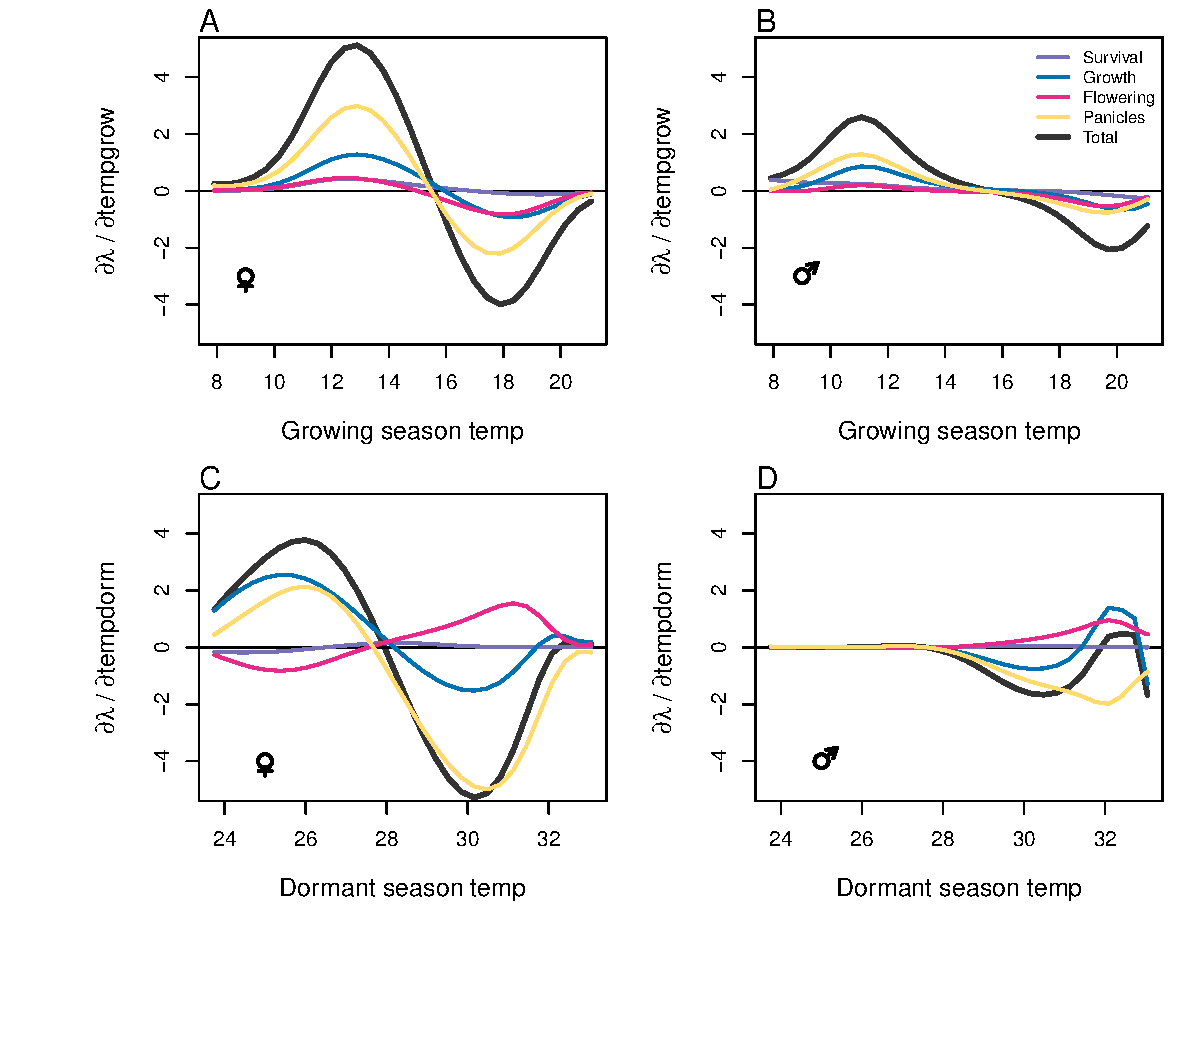
\includegraphics[width=0.95\linewidth]{Figures/LTRE_Temperature.pdf}
  \caption{XXX}
  \label{fig:LTRETemp}
  \end{center}
\end{figure}


\subsection*{Climatic change induce range shifts}
Across species niche population persistence was maximized at higher temperature during the dormant season ( 27 to 31) and intermediate temperature during the growing season (11 to 20). 
Our demographically based range predictions broadly captured the known distribution of the species (Fig. 1). 
More specifically, the predicted population viable ($\lambda>1$) matches the presence and absence of the species. 
Furthermore, viable populations of \emph{P. arichnifera} were only predicted at the center of the range for current climatic conditions (Fig1).
Future and past projections of climate change showed a north-west range shift compared to current distributions. 
Although \emph{P. arichnifera} was predicted to have suitable habitat in the center of the range under the current climate, future warming is predicted to reduce much of the suitable habitat in the southern part (Figure). 

\begin{figure}[H]
  \begin{center}
    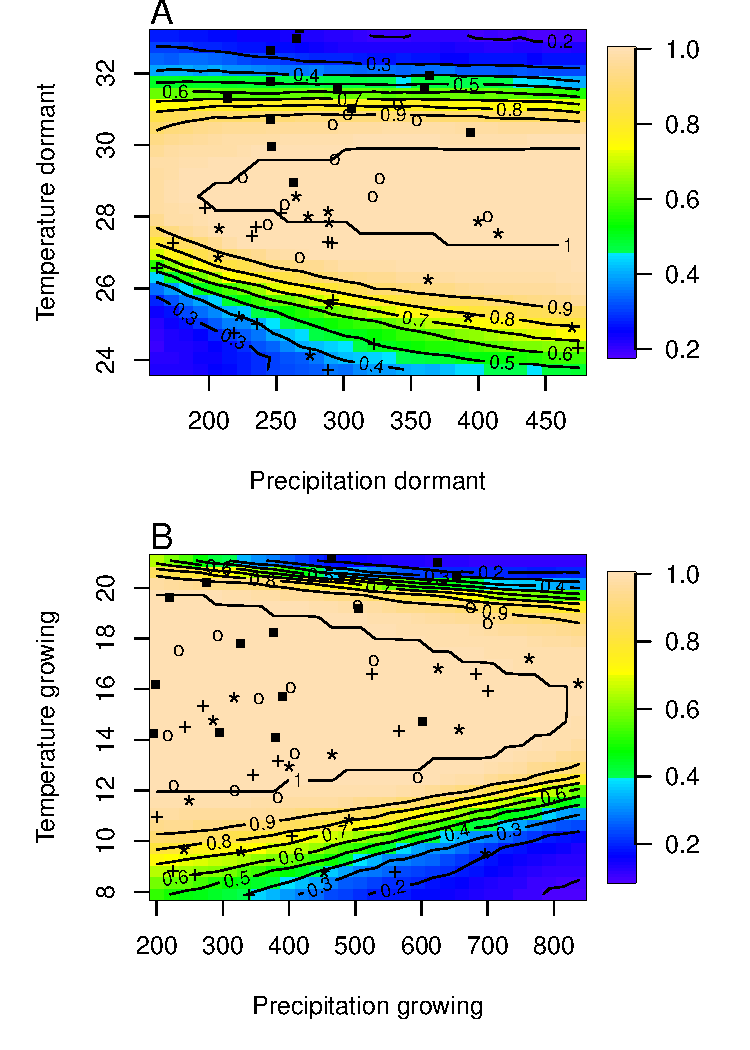
\includegraphics[width=0.85\linewidth]{Figures/niche.pdf}
  \caption{Predicted niche shift for past, present and future climate conditions based on Pr ($\lambda \geq 1$). Niche of dormant season (A), Niche of growing season (B). Contours show predicted probabilities of self- sustaining populations Pr ($\lambda \geq 1$) conditional on precipitation and temperature of the dormant and growing season."+" Past, "*" Current,"o" RCP 45,"." RCP 85}
  \label{fig:niche}
  \end{center}
\end{figure}

\begin{figure}[H]
  \begin{center}
    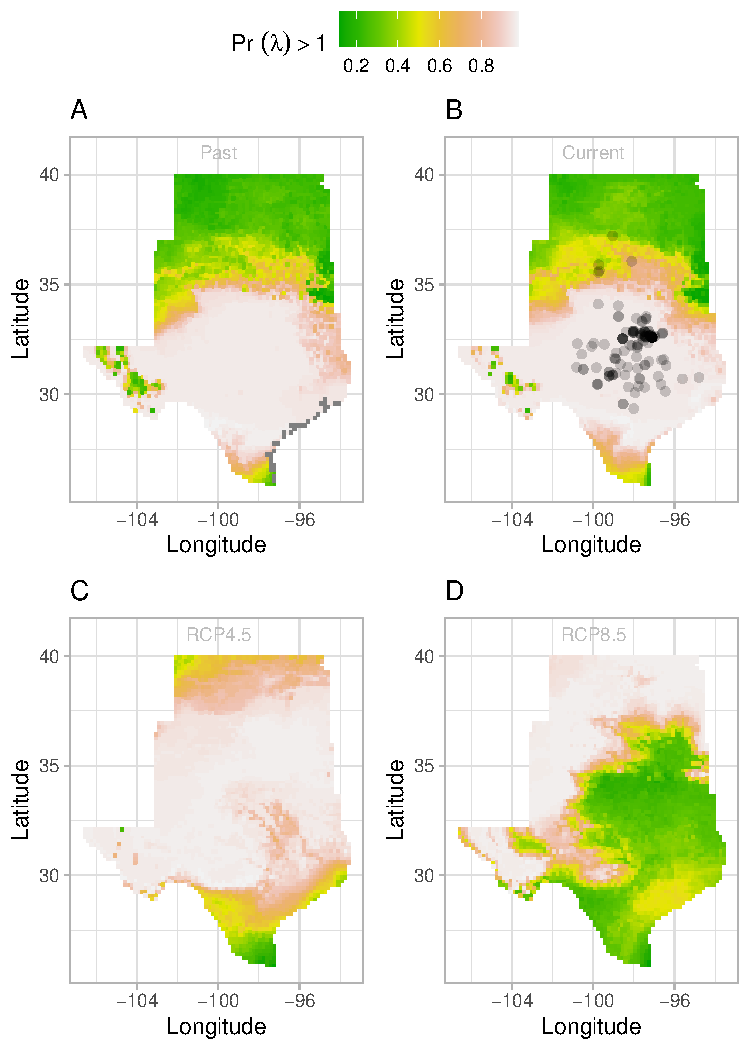
\includegraphics[width=0.75\linewidth]{Figures/Fig_geoPrlambdaprojection.pdf}
  \caption{Past (A), Current (B), Future (2070–20100) (C and D) predicted range shift based on population growth rate using the two sex model. Future projections were based on MIROC. The black circles on panel B indicate all known presence points collected from GBIF from 1990 to 2019, which corresponds to the current condition in our prediction.  The occurrences of GBIFs are distributed inwith higher population fitness habitat ($\lambda$ > 1) , confirming that our study approach can reasonably predict range shifts. }
  \label{fig:geoprojmiroc}
  \end{center}
\end{figure}

\begin{figure}[H]
  \begin{center}
    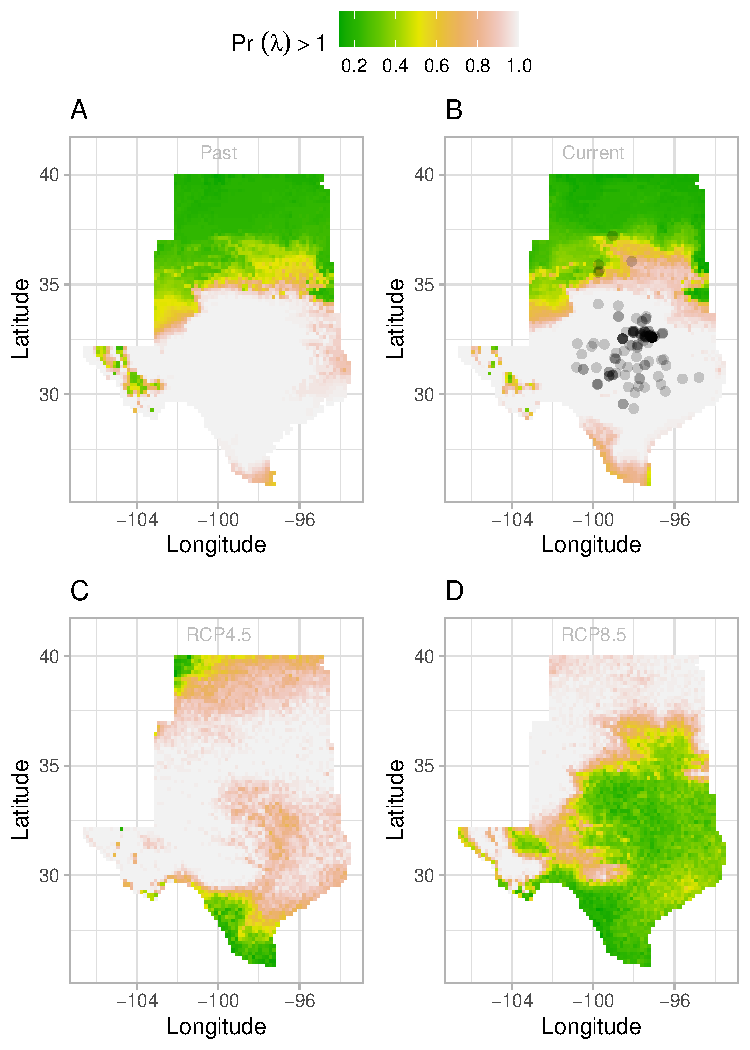
\includegraphics[width=0.75\linewidth]{Figures/Fig_geoPrlambdaprojection_fd_miroc.pdf}
  \caption{Past (A), Current (B), Future (2070–20100) (C and D) predicted range shift based on population growth rate using the female dominant model. Future projections were based on the average population growth rate in four GCMs. The black circles on panel B indicate all known presence points collected from GBIF from 1990 to 2019, which corresponds to the current condition in our prediction.  The occurrences of GBIFs are distributed inwith higher population fitness habitat ($\lambda$ > 1) , confirming that our study approach can reasonably predict range shifts. }
  \label{fig:geoprojfdmiroc}
  \end{center}
\end{figure}

\section*{Discussion}
Three general patterns emerged from our analysis. First, our Bayesian mixed effect model predicts that seasonal climate (temperature and precipitation) affects sex-demographic processes in distinctive and contrasting ways.
While climate has a significant effect on the probability of survival and growth, it has no effect on the number of panicles. Second, future climate, by increasing seasonal temperature, will lead to decline in population viability and favor range shifts. 
Third, using only one sex to forescat range shifts of dioecious under climate change could lead to an underestimation of the impact of  climate change on species.


Our results indicate a sex-specific demographic response to climate change. 
Females have higher survival rate and fertility rate than males. 
This result is not unique to our study system and has been observed in a range of abiotic pollen dispersal species across climatic gradien ts \citep{welbergen2008climate,zhao2012sex,sasaki2019complex}. 
Several hypotheses could explain the observed demographic advantage of females over males for survival and flowering and the opposite for growth and number of panicles.
First, the trade-off between fitness traits (survival, growth fertility) due to resource limitation could explain such a result \citep{cipollini1994sexual,freeman1976differential}.
For most species, females often pay more for reproduction than males due to the requirement to develop seeds and fruits. 
However, several studies reported a higher cost of reproduction for males in wind pollinated species due to the larger amounts of pollen they produce \citep{burli2022environmental,hultine2016climate,cipollini1994sexual,bruijning2017surviving,field2013comparative}.

Under current conditions, most population across the range are viable.
This result could be explained by two hypotheses.
First, demographic compensation whereby an increase of one vital rate is coupled with a decrease of another vital rate could explain a viable population in harsh conditions at the range edge \citep{doak2010demographic,villellas2015demographic}. 
In our system, a decrease in fertility survival rate was counterbalanced by an increase in survival rate, preventing the population growth rate from declining even at range edge for the growing season.
Second, local adaptation at the edge of the range explains the viable population throughout the range \citep{miller2022two}. 
Our study was based on a common garden experiment; therefore, individuals planted in climatic conditions that are similar to their source populations climatic conditions suffer less from stressful environmental conditions.
The question to ask is whether the local population could help the population at the edge to buffer against climate.
Unfortunately, our model does not shed light on the role of local adaptation in species response to climate change. 
Moreover, our future projections require extrapolation to warmer or colder conditions than observed in our experiment and subsequently should be interpreted with caution. 
Despite this limitation, our model did well in predicting the suitable area for the species. 

Projected future climate by inducing an increase in seasonal temperature will affect population viability. 
Temperature can impact plant populations through different mechanisms. 
Increasing temperature could increase evaporative demand, affect plant phenology and germination rate. 
The potential for temperature to influence these different processes changes seasonally \citep{korner2006significance}. 
In the summer growing season, when the temperature is high, the effect on the water balance should be strong.
In the dormant season, when evaporative demand is low, temperature should have a more important effect on phenology and germination. Because our study species was sensitive to temperatures in the growing season, the former mechanism deserve further attention. 

The reduction in population viability across the range due to climate change will drive a shift to the north range in suitable habitat for the species. 


\newpage
\bibliographystyle{apalike}
\bibliography{Forecasting}
%--------------------------------------------------------------------
\newpage
\clearpage 
\setcounter{equation}{0}
\setcounter{figure}{0}
\setcounter{section}{0}
\setcounter{table}{0}
\renewcommand{\theequation}{S.\arabic{equation}}
\renewcommand{\thetable}{S-\arabic{table}}
\renewcommand{\thefigure}{S-\arabic{figure}}
\renewcommand{\thesection}{S.\arabic{section}}

\centerline{\Large{\textbf{Supporting Information}}}

\section {XX}	

\begin{figure}[H]
		\centering
		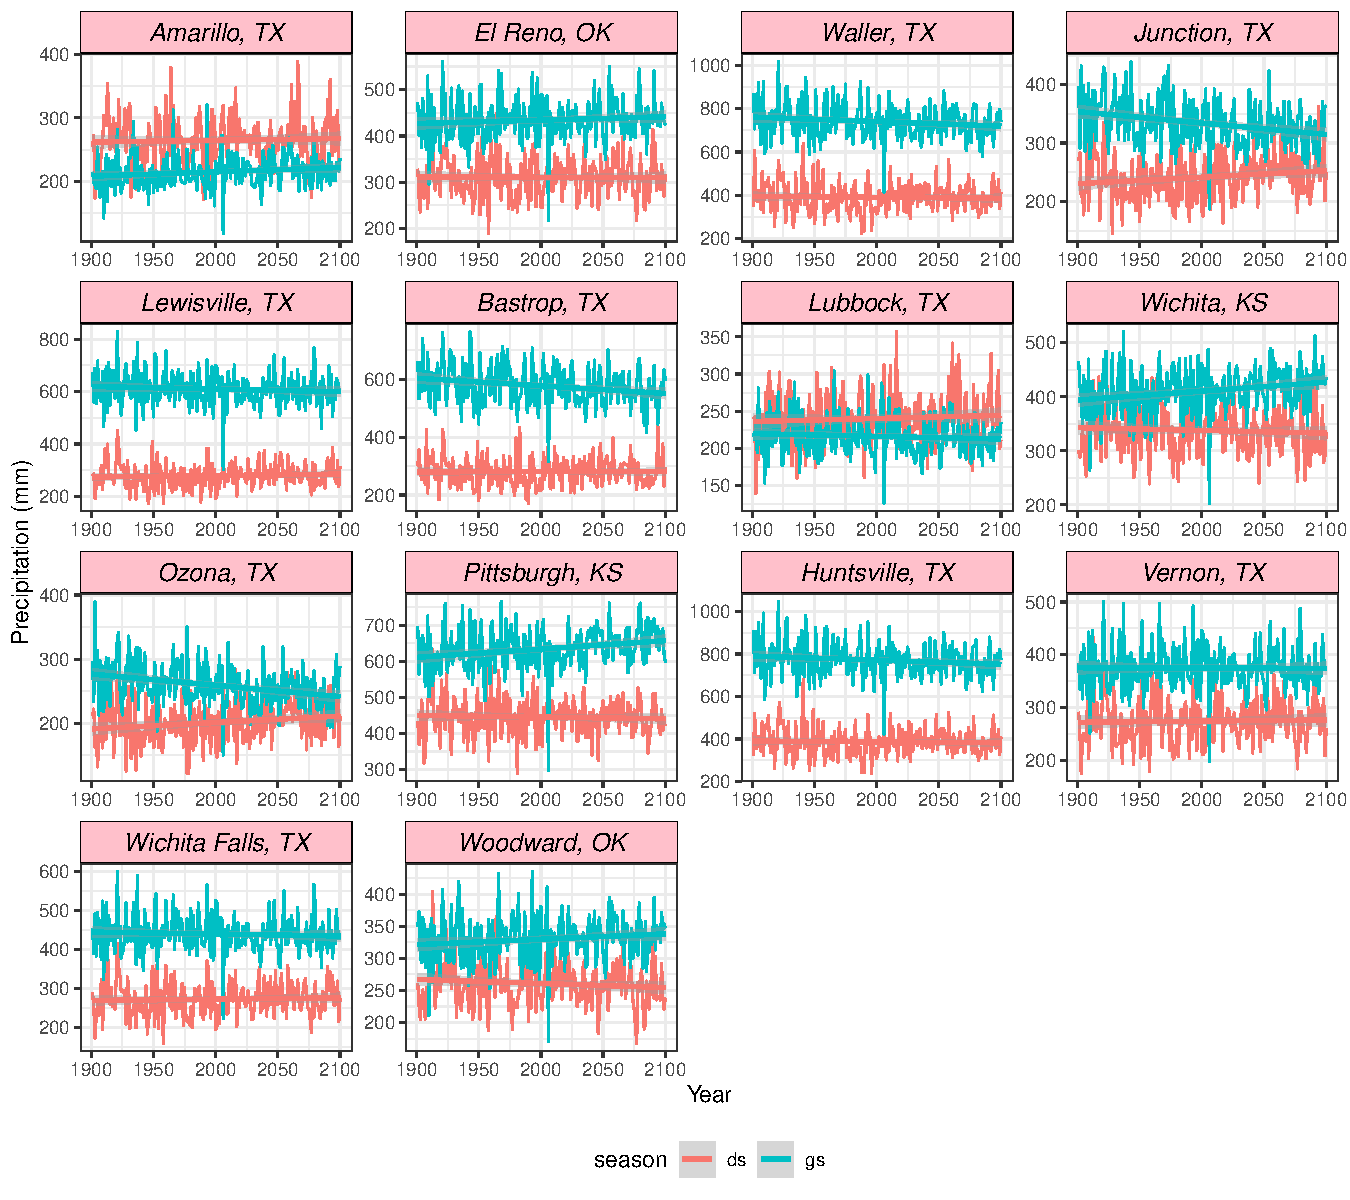
\includegraphics[width=0.95\linewidth]{Figures/fig_pr_past_present_future.pdf}
		\caption{\textbf{Precipitation variation accross the study sites from 1990 to 2100}}
		\label{Sup:pr_variation}
\end{figure}


\begin{figure}[H]
		\centering
		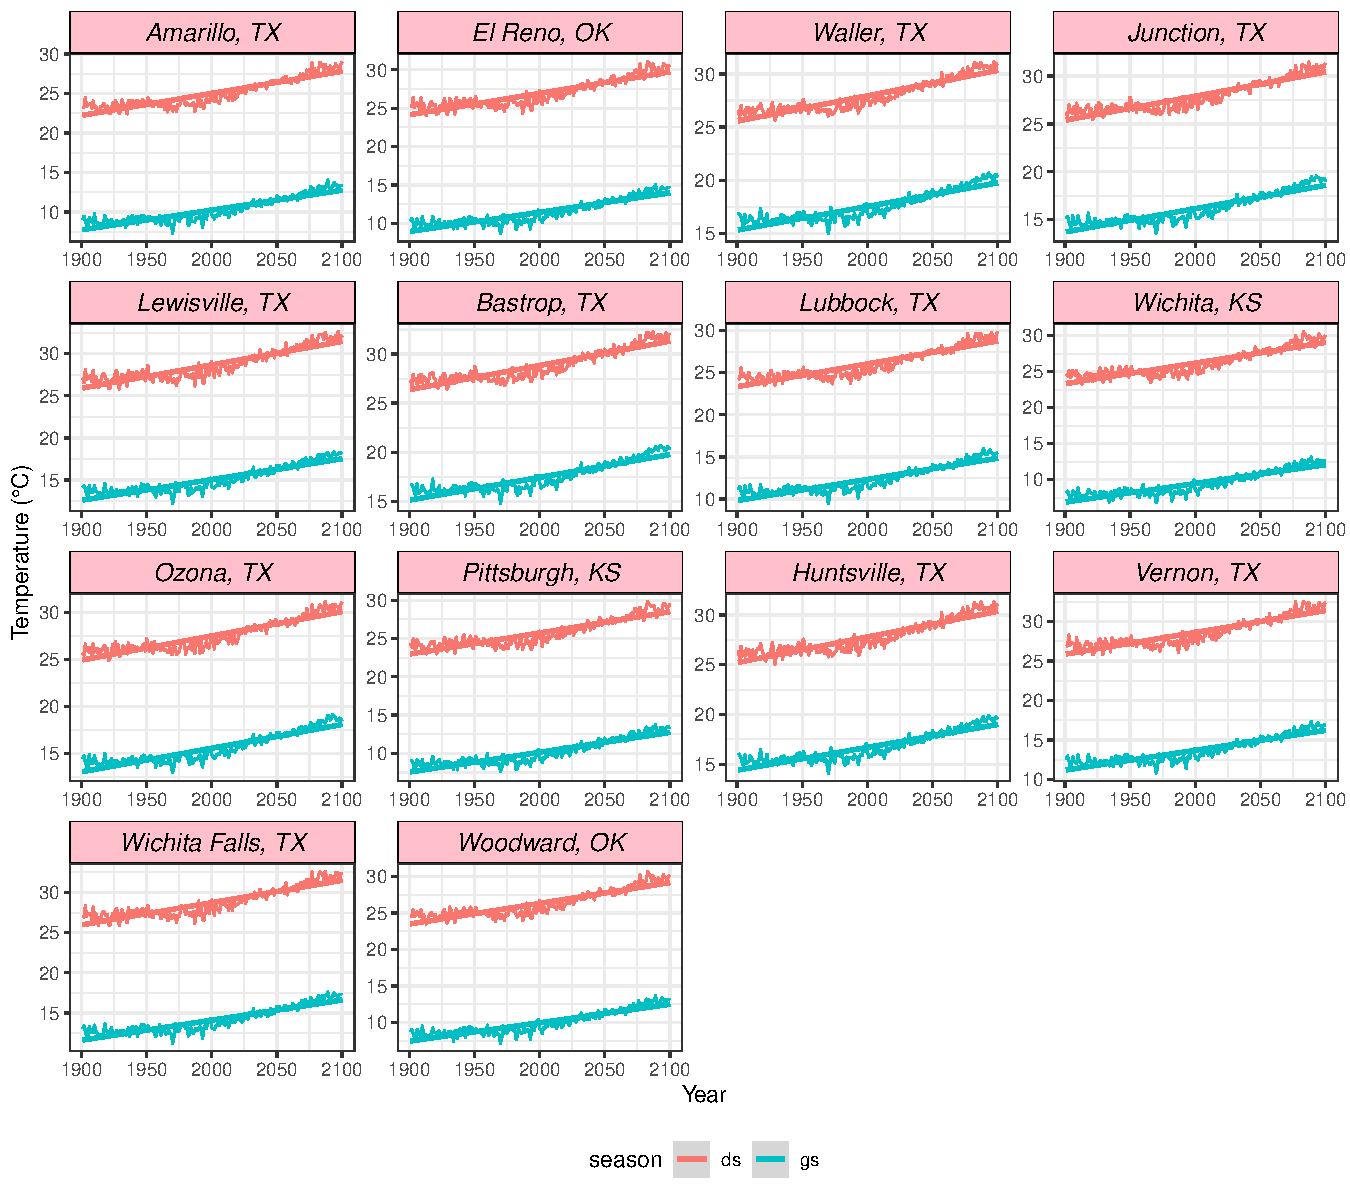
\includegraphics[width=0.95\linewidth]{Figures/fig_tas_past_present_future.pdf}
		\caption{\textbf{Temperature variation accross the study sites from 1990 to 2100}}
		\label{Sup:temp_variation}
\end{figure}




\begin{figure}[H]
		\centering
		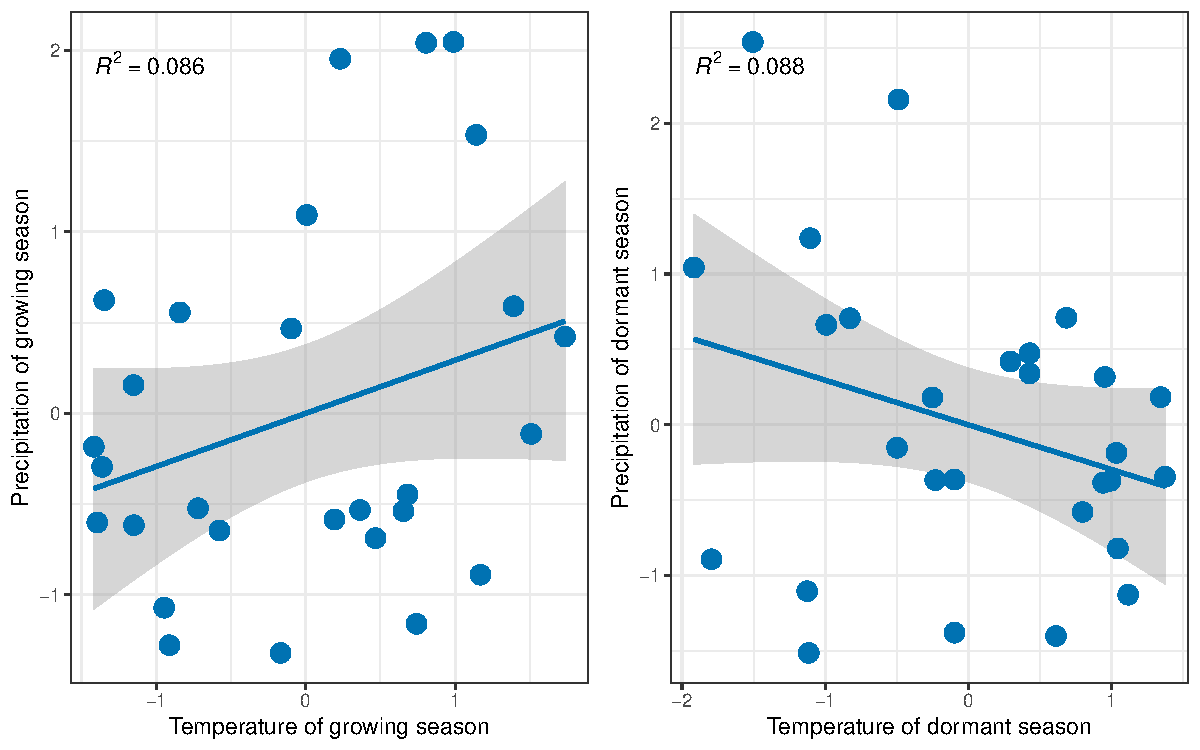
\includegraphics[width=0.95\linewidth]{Figures/Varianceexplained.pdf}
		\caption{\textbf{Relation between precipitation and temperature for each season (growing and dormant).} $R^2$ indicates the value of proportion of explained variance between the temperature and precipitation}
		\label{Sup:Correlation}
\end{figure}
	
\begin{figure}[H]
		\centering
		\includegraphics[width=0.75\linewidth]{Figures/PPC.pdf}
		\caption{\textbf{Consistency between real data and simulated values suggests that the fitted model accurately describes the data}. Graph shows density curves for the observed data (light blue ) along with the simulated values (dark blue). The first column shows the linear models and the second column shows the 2 degree polynomial models.}
		\label{Sup:PPC}
	\end{figure}
	
\begin{figure}[H]
		\centering
		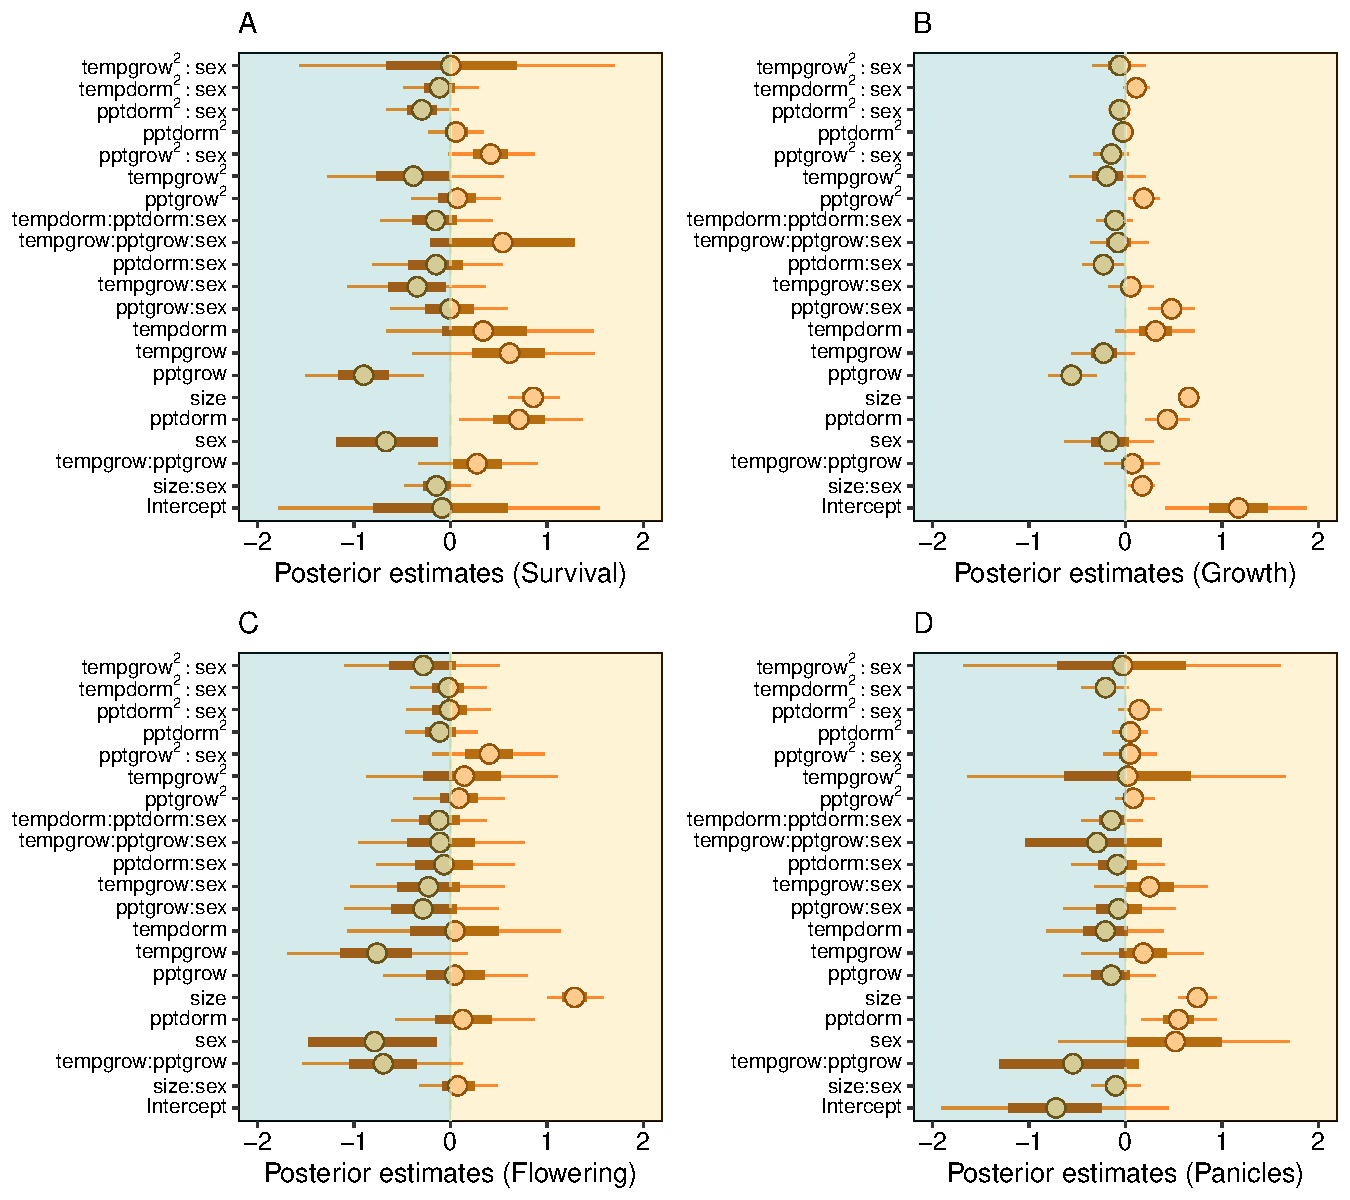
\includegraphics[width=0.95\linewidth]{Figures/Posterior_mean.pdf}
		\caption{\textbf{Mean parameter values and 95\% credible intervals for all vital rates}. }
		\label{Sup:Posterior}
\end{figure}
	
\begin{figure}[H]
  \begin{center}
    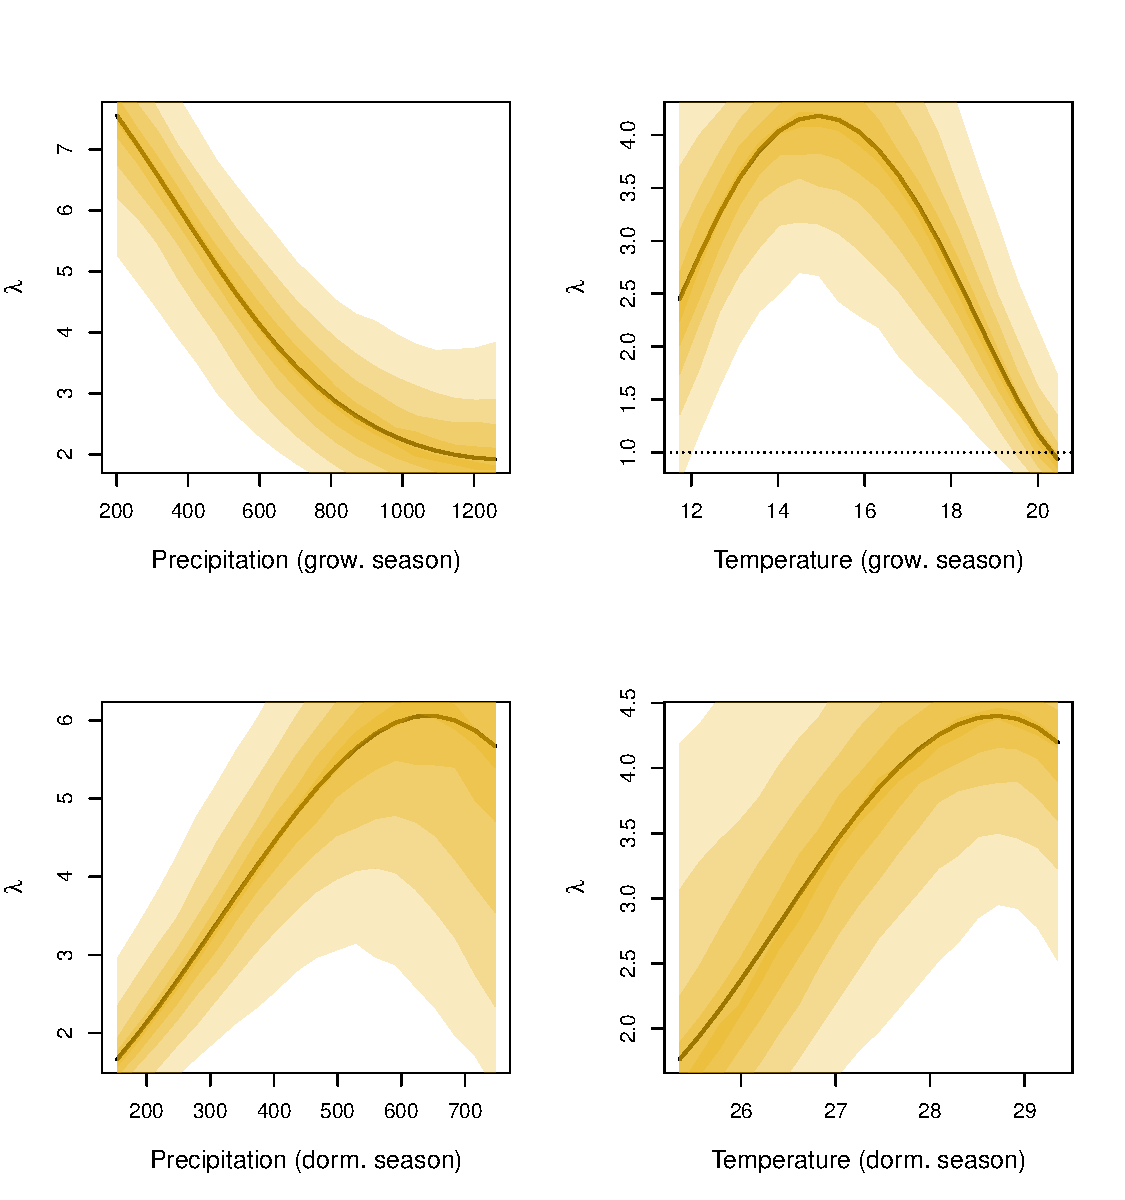
\includegraphics[width=0.95\linewidth]{Figures/lambda_CI.pdf}
  \caption{Population growth rate ($\lambda$) as a function of seasonal climate (2016-2017), predicted by the two-sex matrix projection model that incorporates sex-specific demographic responses to climate with sex ratio-dependent seed fertilization.
We show the mean posterior distribution of $\lambda$ in solid lines, and the 5, 25, 50, 75, and 95\% percentiles of parameter uncertainty in shaded gold color.
The dashed horizontal line indicates the limit of population viability ($\lambda$ = 1)}
  \label{Sup:lambda2sex}
  \end{center}
\end{figure}

\begin{figure}[H]
  \begin{center}
    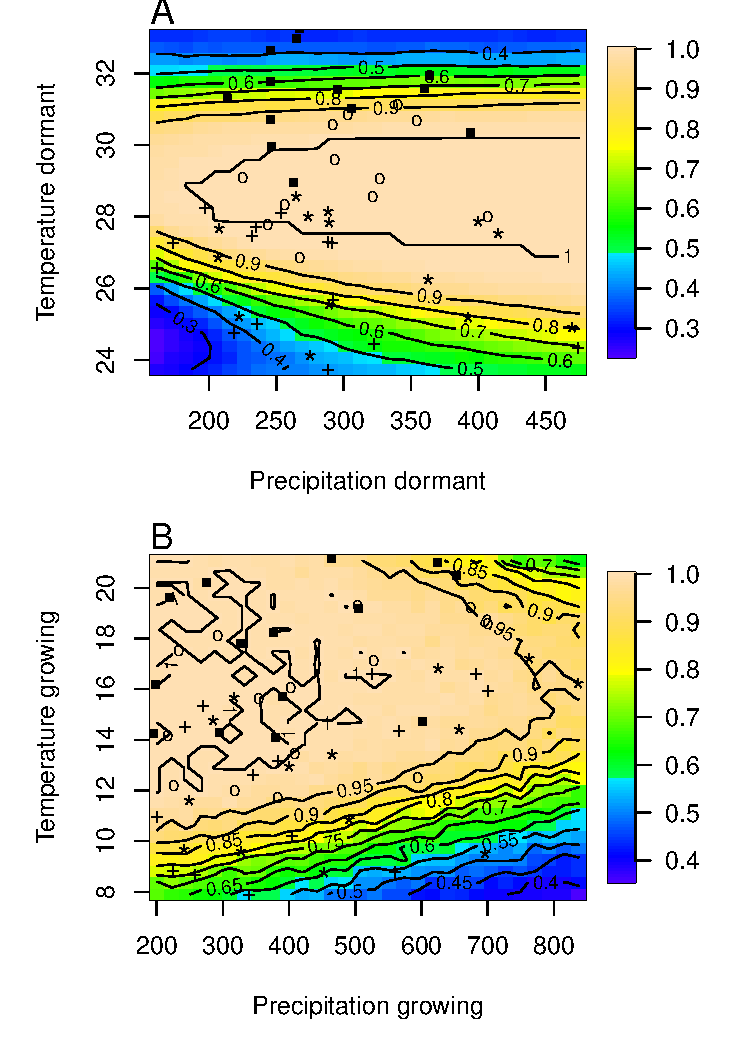
\includegraphics[width=0.78\linewidth]{Figures/niche_female_dominant.pdf}
  \caption{Predicted niche shift for past, present and future climate conditions based on Pr ($\lambda \geq 1$). Niche of dormant season (A), Niche of growing season (B). Contours show predicted probabilities of self- sustaining populations Pr ($\lambda \geq 1$) conditional on precipitation and temperature of the dormant and growing season."+" Past, "*" Current,"o" RCP 45,"." RCP 85}
  \label{fig:geoprojfd}
  \end{center}
\end{figure}

\begin{figure}[H]
  \begin{center}
    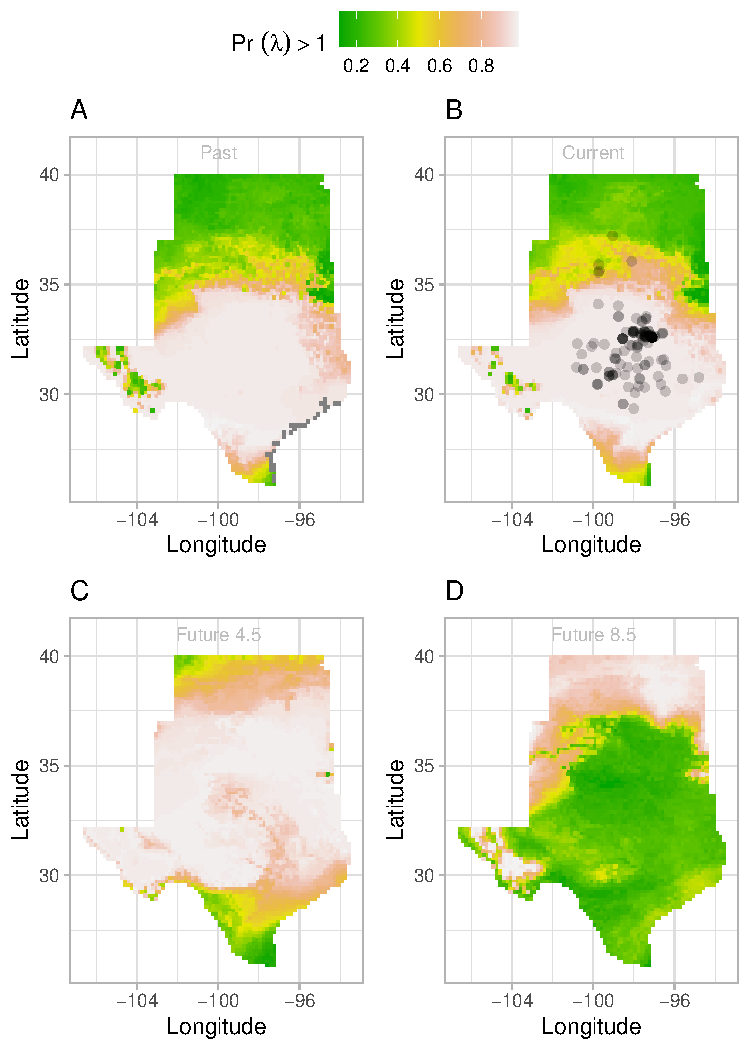
\includegraphics[width=0.78\linewidth]{Figures/Fig_geoPrlambdaprojectioncmc.pdf}
  \caption{Past (A), Current (B), Future CMCM (2070–20100) (C and D) predicted range shift based on population growth rate. Future projections were based on the average population growth rate in four GCMs. The black circles on panel B indicate all known presence points collected from GBIF from 1990 to 2019, which corresponds to the current condition in our prediction.  The occurrences of GBIFs are distributed inwith higher population fitness habitat ($\lambda$ > 1) , confirming that our study approach can reasonably predict range shifts. }
  \label{fig:geoprojcmc}
  \end{center}
\end{figure}

\begin{figure}[H]
  \begin{center}
    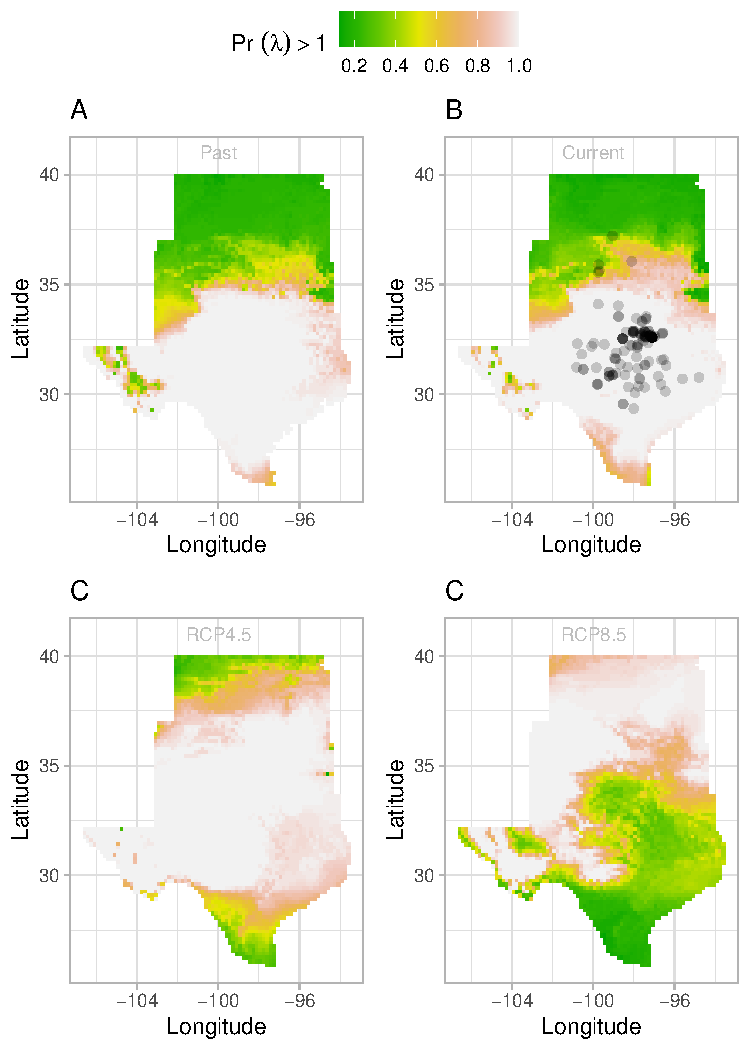
\includegraphics[width=0.78\linewidth]{Figures/Fig_geoPrlambdaprojection_fd_acc.pdf}
  \caption{Past (A), Current (B), Future ACCESS (2070–20100) (C and D) predicted range shift based on population growth rate suing the female dominat model. Future projections were based on the average population growth rate in four GCMs. The black circles on panel B indicate all known presence points collected from GBIF from 1990 to 2019, which corresponds to the current condition in our prediction.  The occurrences of GBIFs are distributed inwith higher population fitness habitat ($\lambda$ > 1) , confirming that our study approach can reasonably predict range shifts. }
  \label{fig:geoproj}
  \end{center}
\end{figure}

\begin{figure}[H]
  \begin{center}
    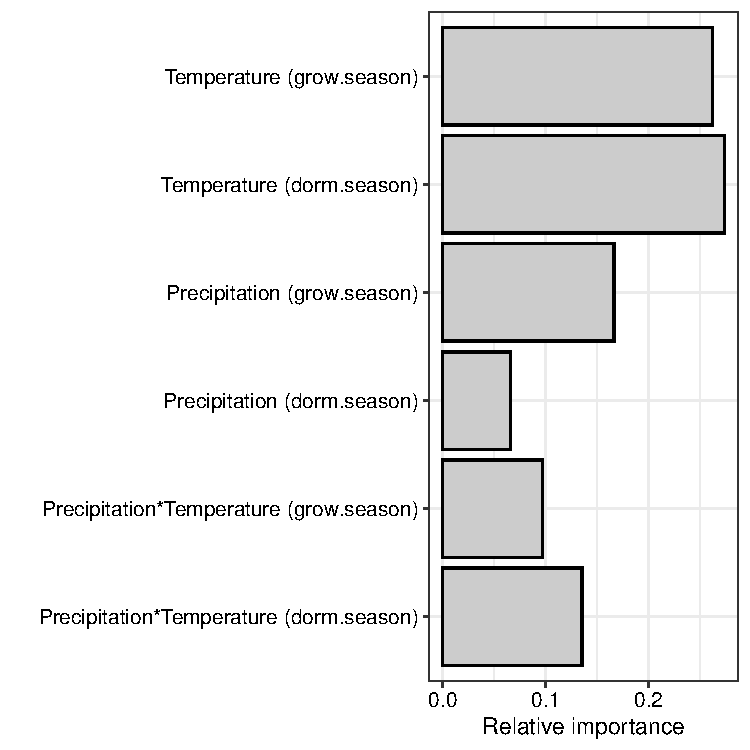
\includegraphics[width=0.85\linewidth]{Figures/Fig_LTRE.pdf}
  \caption{XXX}
  \label{Sup:LTRE}
  \end{center}
\end{figure}

\begin{figure}[H]
  \begin{center}
    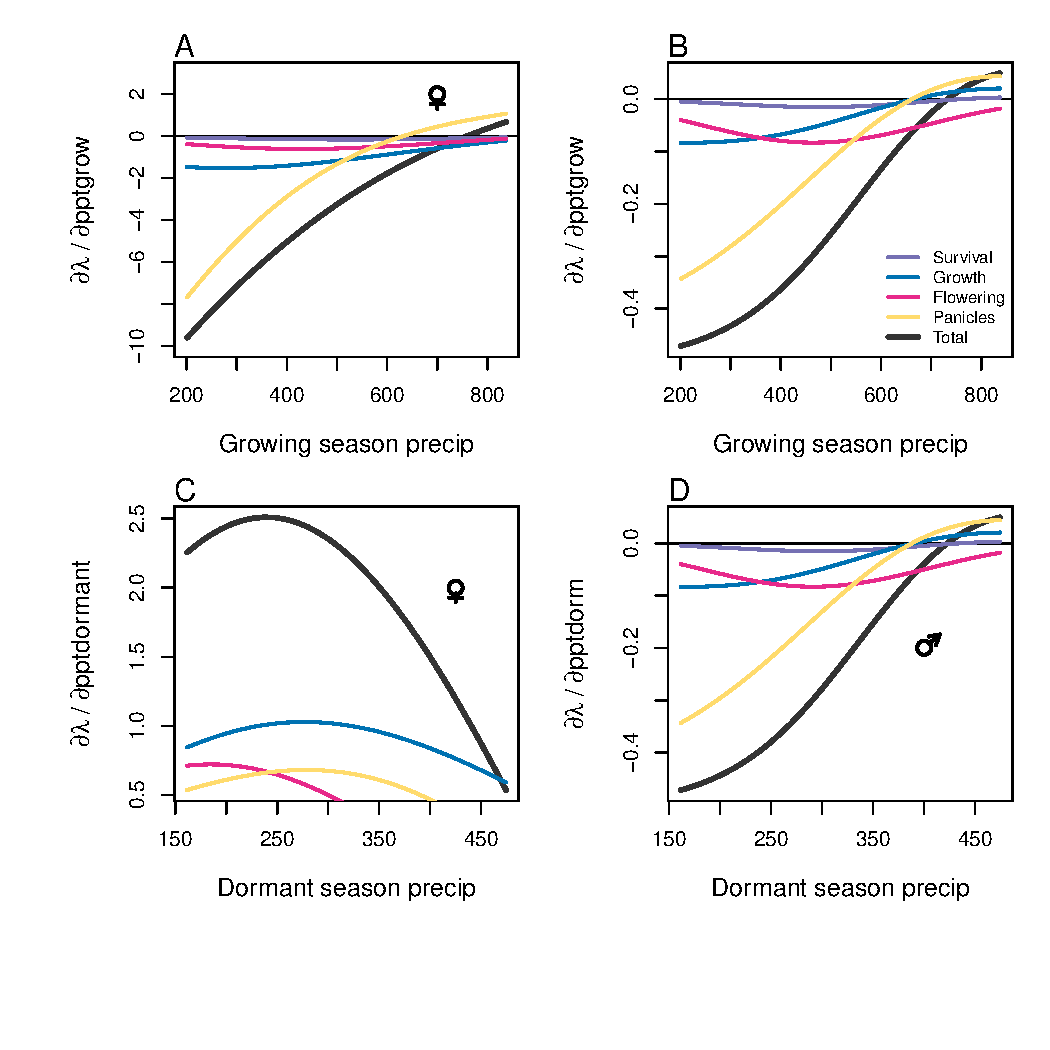
\includegraphics[width=0.85\linewidth]{Figures/LTRE_Precipitation.pdf}
  \caption{XXX}
  \label{Sup:LTREPPT}
  \end{center}
\end{figure}


\end{document}
